\documentclass[palatino,nosec,nobuildate]{Docencia}


\title{Examen modelo con solución (4ºE)}

\author{Departamento de Matemáticas}
\date{17/18}


% Paquetes adicionales

\usepackage[author={Víctor de Juan, 2017}]{pdfcomment}

\usepackage{pgf,tikz}
\usetikzlibrary{arrows}


\definecolor{qqttcc}{rgb}{0,0.2,0.8}
\definecolor{qqqqff}{rgb}{0,0,1}
\definecolor{cccccc}{rgb}{0.8,0.8,0.8}


\makeatletter
\newcommand{\annotate}[2][]{%
\pdfstringdef\x@title{#1}%
\edef\r{\string\r}%
\pdfstringdef\x@contents{#2}%
\pdfannot
width 2\baselineskip
height 2\baselineskip
depth 0pt
{
/Subtype /Text
/T (\x@title)
/Contents (\x@contents)
}%
}
\makeatother



\usepackage{eso-pic}
\newcommand\BackgroundPic{%
\put(0,0){%
\parbox[b][\paperheight]{\paperwidth}{%
\vfill
\centering

\includegraphics[width=\paperwidth,height=\paperheight,%
keepaspectratio]{../../../../BWLogo.jpeg}%
\vfill
}}}





\begin{abstract}
Solución del primer parcial de la segunda evaluación.

\nota{Estos ejemplos no están exentos de erratas. En caso de descubrir alguna, por favor, comunicarlas.}
\end{abstract}

% --------------------
\newcommand{\cimplies}{\text{\hl{$\implies$}}}

\begin{document}
\pagestyle{plain}
%\maketitle

\AddToShipoutPicture{\BackgroundPic}

\begin{problem} (1.5 puntos)

Calcula las siguientes razones trigonométricas:

\ppart $\cos\left(\rfrac{-3π}{4}rad\right)$
\ppart $\cosec(1050º)$
\solution

\spart $\cos(-\rfrac{-3π}{4}rad) = \cos(-135º) = \cos(135) = -\cos(45) = -\rfrac{\sqrt{2}}{2}$

\spart $$\cosec(1050º)=\frac{1}{\sen(1050º)} = \frac{1}{\sen(1050-720)} = \frac{1}{\sen(330)} = -\frac{1}{\sen(360-330)} = -\frac{1}{\sen(30)} = -\frac{1}{\rfrac{1}{2}} = -2$$


\end{problem}

\begin{problem}(1.5 puntos)
Sabiendo que $\tg(α) = +\sqrt{8}$ y que $180º<α<270º$, halla las demás razones trigonométricas. Ten en cuenta el cuadrante para el signo de cada razón trigonométrica. Deja los resultados en forma de fracción.

\solution

\[
	\left.
	\begin{array}{c}
		\tg(α) = \sqrt{8}\\
		\cotg(α) = \frac{1}{\tg(α)}
	\end{array}
	\right\} \to \tg(α) = \frac{1}{\cotg(α)} = \frac{1}{\sqrt{8}} = \frac{\sqrt{8}}{8}
\]

\[
	\left.
	\begin{array}{c}
		\tg(α) = \sqrt{8}\\
		\tg^2(α) + 1 = \sec^2(α)
	\end{array}
	\right\} \to \sec^2(α) = \left(\sqrt{8}\right)^2 + 1  \implies \sec(α) = \sqrt{9}
\]

Como está en el tercer cuadrante, la secante es negativa. Por lo tanto, elegiremos la solución negativa de la raíz: $\sec(α) = -3$

\[
	\left.
	\begin{array}{c}
		\sec(α) = -3\\
		\sec(α) = \frac{1}{\cos(α)}
	\end{array}
	\right\} \to \cos(α) = -\frac{1}{3}
\]

\[
	\left.
	\begin{array}{c}
		\tg(α) = \frac{\sen(α)}{\cos(α)}\\
		\cos(α) = -\frac{1}{3}
	\end{array}
	\right\} \to \sen(α) = \cos(α)·\tg(α) = -\frac{1}{3}\sqrt{8} = -\frac{\sqrt{8}}{3}
\]


\[
	\left.
	\begin{array}{c}
		\sen(α) = -\frac{\sqrt{8}}{3}\\
		\cosec(α) = \frac{1}{\sen(α)}
	\end{array}
	\right\} \to \cosec(α) = -\frac{3}{\sqrt{8}} = -\frac{3\sqrt{8}}{8}
\]



\end{problem}


\begin{problem} (1 punto)
Las dos ramas de un compás forman $60º$ y tiene las puntas abiertas a una distancia de 12cm. ¿Cuánto mide cada rama?

\solution

El compás forma un triángulo equilátero, por lo que las ramas miden también 12 cm.

\end{problem}

\begin{problem} (2 pto) 2 amigos quieren medir la altura de
un edificio de 4 plantas iguales. Uno se
sitúa a √3m del edificio (P1) y ve el tejado
del edificio con un ángulo de $30º$. ¿Cuál es
la altura del edificio? ¿A qué distancia se
sitúa el otro (P2) si ve la separación entre la
2a y 3a planta con $45º$?

\solution

\begin{figure}[h]
\centering
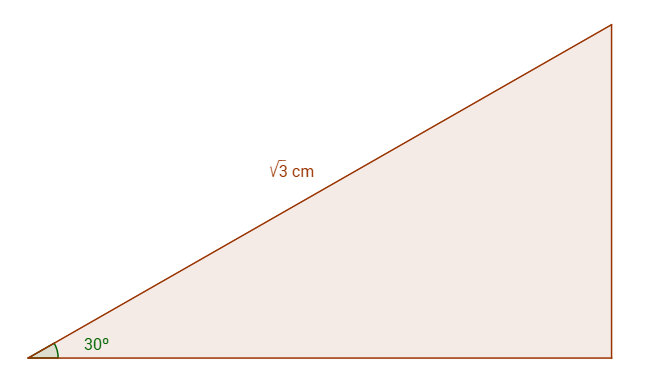
\includegraphics[scale=0.5]{Triang}
\end{figure}

La altura del edificio se calcula:

\[
	\tg(α) = \tg(30º) = \frac{h}{\sqrt{3}} \implies h = \sqrt{3}\frac{\sqrt{3}}{3} = 1m
\]

\textit{El resultado es poco realista, ya que los números debían ser sencillos al no permitir calculadora.}

Si 4 plantas miden 1m, 2 plantas mediran 0.5 metros. 

\[
	\tg(β) = \tg(45º) = \frac{h_2}{x} \implies x = \frac{h_2}{\tg{45}} = \frac{0.5}{1} = \frac{1}{2}m
\]


\end{problem}

\begin{problem} (1.5 pto.)

Resuelve la siguiente ecuación trigonométrica: $\sec x = \sqrt{2}$

\solution

\[\sec x = \rfrac{1}{\cos x}\]

Buscamos cuadrantes en los que el coseno sea positivo, es decir $I$ y $IV$.

Por otro lado:

\[
	\sec x = \sqrt{2} \dimplies \frac{1}{\cos(x)} = \sqrt{2} \dimplies \cos(x) = \frac{1}{\sqrt{2}} = \frac{\sqrt{2}}{2} 
\]

Los ángulos buscados son $45º$ y, pasando al cuarto cuadrante: $360-45 = 315º$

\[
	x_1 = 45º + 360ºk\;\;,\;\; ∀k∈ℤ
\]
\[
	x_2 = 315º + 360ºk\;\;,\;\; ∀k∈ℤ
\]

\end{problem}

\begin{problem}
Resuelve las siguientes inecuaciones:

\ppart 1,5pto.

\[
	\frac{12-3x}{x+2}≤1
\]

\ppart 1pto

\[
	\left\{
		\begin{array}{c}
			3x+y<2\\
			y≥x+2
		\end{array}
	\right\}
\]

\solution

\spart 
\[
	\frac{12-3x}{x+2} - 1 ≤ 0 \dimplies \frac{12-3x-x-2}{x+2} ≤ 0 \dimplies \frac{10-4x}{x+2}≤0
\]

Construimos la tabla
\[
\begin{array}{ccccc}
&(-\infty,-2)&(-2,2.5)&(2.5,\infty)\\
(-4x+10)&+&+&-\\
(x+2)&-&+&+\\
\frac{(x-2)(x-3)}{x+2} & - & + & - \\
\end{array}
\]

\textbf{Solución:} $(-\infty,-2) ∪ [2.5,\infty)$

\spart 

\begin{figure}[h]
\centering
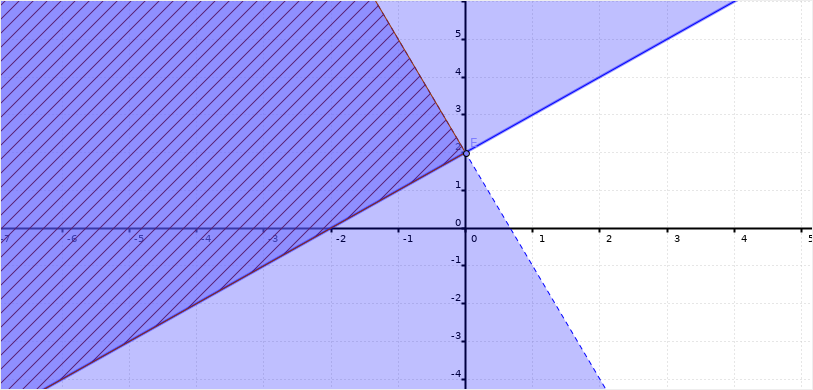
\includegraphics[scale=0.45]{inec}
\end{figure}

\end{problem}

\end{document}
